\documentclass[format=sigconf,nonacm,screen]{acmart}
\usepackage{amsmath}
\usepackage{subcaption}

\setcopyright{none}

\hyphenation{Zoo-Keep-er}
\hyphenation{DNS-Zoo}
\hyphenation{get-Child-ren}
\hyphenation{go-rou-tine}
\hyphenation{Open-DNS}

\newcommand{\dnszoo}{\textsf{DNSZoo}}
\newcommand{\dnszooch}{\textsf{DNSZoo-CH}}
\newcommand{\dnszoor}{\textsf{DNSZoo-R}}

\begin{document}

\title{DNSZoo: Replicated DNS Cache Service backed by ZooKeeper-based Membership Management}

\author{Haishan Gao}
\email{hsgao@stanford.edu}
\affiliation{%
  \institution{Stanford University}
  \city{Stanford}
  \state{CA}
  \country{USA}
}

\author{Timothy Gu}
\email{timothygu@stanford.edu}
\affiliation{%
  \institution{Stanford University}
  \city{Stanford}
  \state{CA}
  \country{USA}
}

\author{Zhongyang Liu}
\email{jerrylzy@stanford.edu}
\affiliation{%
  \institution{Stanford University}
  \city{Stanford}
  \state{CA}
  \country{USA}
}

\begin{abstract}    
\small We design and implement a distributed DNS cache service with replicated cache in a hierarchical structure. Our system demonstrates high availability, horizontal scalability, and robustness to withstand server node failures. It supports instant server membership management to add and remove nodes dynamically. We propose a tailored design of load balancing strategy and consensus protocol in our system that relaxes the consistency requirement to achieve high availability and partition tolerance. The system is deployed and fully tested on Amazon EC2. We measure its latency, throughput and ability to tolerate node failures and validate it outperforms Google DNS service (8.8.8.8) on the latency metric in a local area network environment.
\end{abstract}

\maketitle

\fontsize{11}{11}\selectfont

\section{Introduction}
The Domain Name System (DNS) is a naming database system used to translate human readable internet domain names into Internet Protocol (IP) addresses. DNS serves as an indispensable entry point to modern network architecture. Its services need to be highly accurate and widely available to enable users worldwide to access online contents and email services. DNS service outage leads to the total inability for regular users to reach any websites and high latency of DNS service will also impact user experience in participating in web activities. Furthermore, the DNS architecture needs to be able to extend its scale to cope with the growing traffic of web usage nowadays.

A widely adopted design to satisfy high availability and scalability is to maintain multiple servers to answer to the domains in the same hash range. Hence, a request routing and load balancing algorithm is needed to deliver user queries evenly to the servers. A consensus protocol is needed to ensure the eventual consistency of the cached records over the servers. Though the requirements and functionalities of the DNS server have been well understood, the design of its underlying algorithms and policies has been an active research area \cite{1999redirection,2004cdn,2004democratizing,2020dns} for different use cases with varying geographic proximity and content delivery specialities.

For normal users, public DNS services, such as Cloudflare, Google, OpenDNS, etc., are more than enough. However, when we develop large-scale distributed systems that heavily utilize DNS services, such as web crawlers, we cannot afford to use public DNS directly due to lack of latency guarantees and the threat of getting throttled or even banned. Therefore, a custom internal DNS caching service like ours comes in handy to address those two serious concerns.

In this paper, we present \dnszoo{}, a distributed Domain Name System with high availability, scalability and non-Byzantine fault tolerance. Its key design is to use ZooKeeper for server membership management, as well as tailored request routing and consensus protocols to provide high availability. Based on the overall requirements, we propose and design two variants of \dnszoo{}, \dnszooch{} (using Consistent Hashing) and \dnszoor{} (using Raft-backed storage). Both variants implemented are available in open-source code. We deploy and measure the performance of \dnszooch{} on Amazon EC2.


% We designed two competing DNS caching systems,
% DNSZoo-CH (using Consistent Hashing) and
% DNSZoo-R (using Raft), and fully implemented
% DNSZoo-CH.

\section{Background}

\subsection{Domain Name System}

DNS \cite{rfc1034,rfc1035} is a global distributed system for storing information about domain names. DNS supports a wide variety of information, but of particular interest to us is the \emph{A record} which contains mappings between a domain and IPv4 addresses, and the \emph{CNAME record} which defines an alias for another domain name. For this project we consider only A and CNAME records, since they are essential for browsing the World Wide Web.

DNS contains an astoundingly large number of domain names (on the order of hundreds of millions in registered domains alone, not including subdomains). However, a small number of them (typically those corresponding to popular websites) are accessed with disproportionate frequency. Prior studies \cite{1992dnscaching,2002dnscaching} conclude that locality of reference effectively predicts future queries, which supports the use of caches containing recently and frequently fetched records. To support caching, each DNS record contains a Time-To-Live (TTL) field defining the time span for which the record can be used (typically on the order of minutes to hours). We use the TTL field to determine the length of time we are allowed to cache a particular record -- or if we should attempt to cache it at all.

\subsection{Consistent Hashing}

Consistent Hashing \cite{1997consistenthashing,2001chord} is a mechanism to evenly distribute work across a set of servers, while also allowing adding or removing servers. In the context of \dnszooch{}, each node serves as the secondary cache for a range of potential hash values, and Consistent Hashing allows easy discovery of the responsible server for a particular query.

To maintain a high cache hit rate through reconfiguration, for each update to the server set, we wish to minimize the number of changes to the hash ranges. We specifically use Consistent Hashing with Bounded Loads \cite{2016chbl}, which guarantees an expected constant number of DNS query ownership changes.

\subsection{Raft}

Raft \cite{2014raft} is a consensus protocol implementing a replicated state machine. Raft uses a strong leader, where all proposals must be sent to the leader and then broadcast to individual nodes. In \dnszoor{}, we work around this potential bottleneck by allowing lock-free reads and only use Raft for cache broadcasting.

\subsection{ZooKeeper}
ZooKeeper \cite{2010zookeeper} is an open-source coordination service commonly used in the industry. We use ZooKeeper for various control operations such as service discovery and leader election that require linearizability guarantees.
While we could have implemented similar functionality using Raft ourselves, we note that our usage of ZooKeeper does not fall on the critical path of DNS queries. Additionally, the client library provides a convenient event-driven API (e.g., watches \cite{2010zookeeper}) that make implementing a number of synchronization primitives much easier than manually with Raft. Finally, since our usage of ZooKeeper is confined to a module separate from actual handling DNS queries, it is relatively easy to switch to a different coordination system (e.g., Chubby \cite{2006chubby}) as needed.

\section{Design}

\begin{figure*}[t]
\vspace*{-\baselineskip}
\centering
    \subcaptionbox{Overall Architecture \label{fig:overall}}{%
    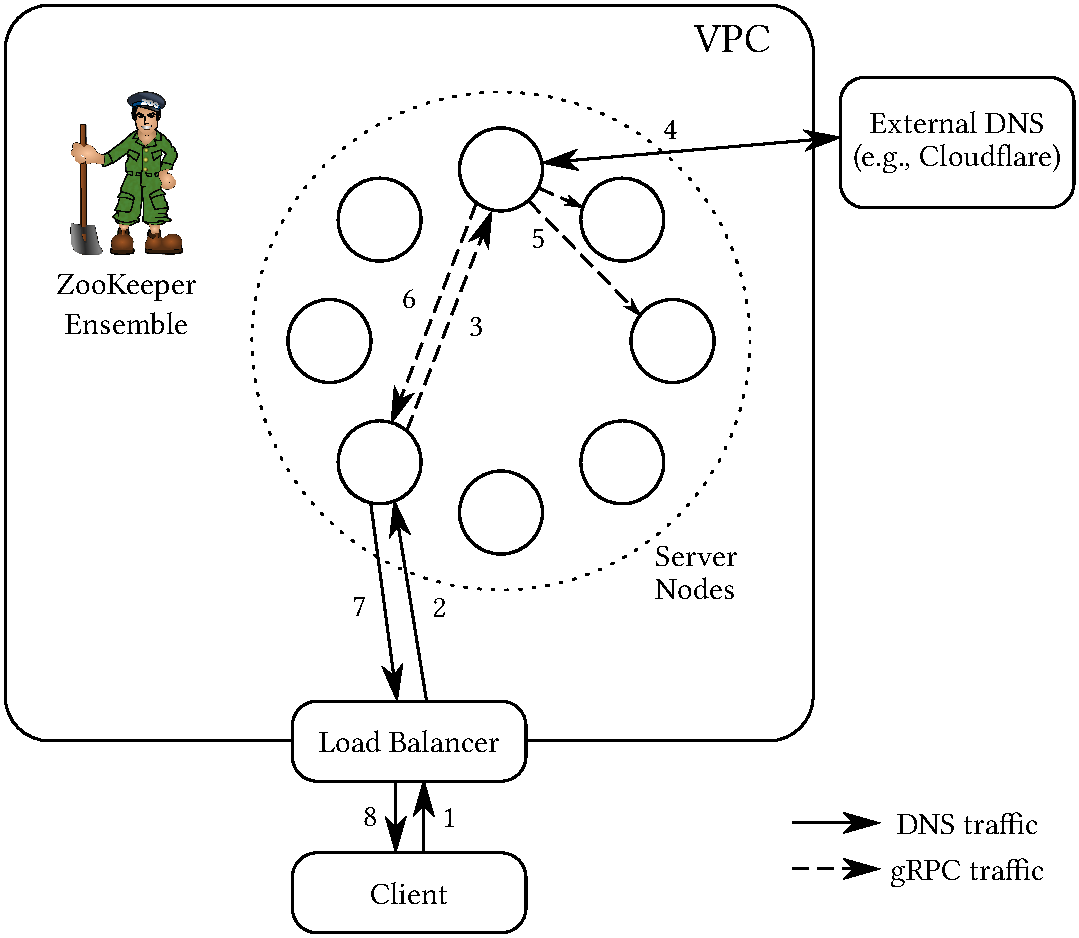
\includegraphics[width=0.35\textwidth]{overall.pdf}}
    \hspace{2em}
    \subcaptionbox{Internal Organization \label{fig:internal}}{%
    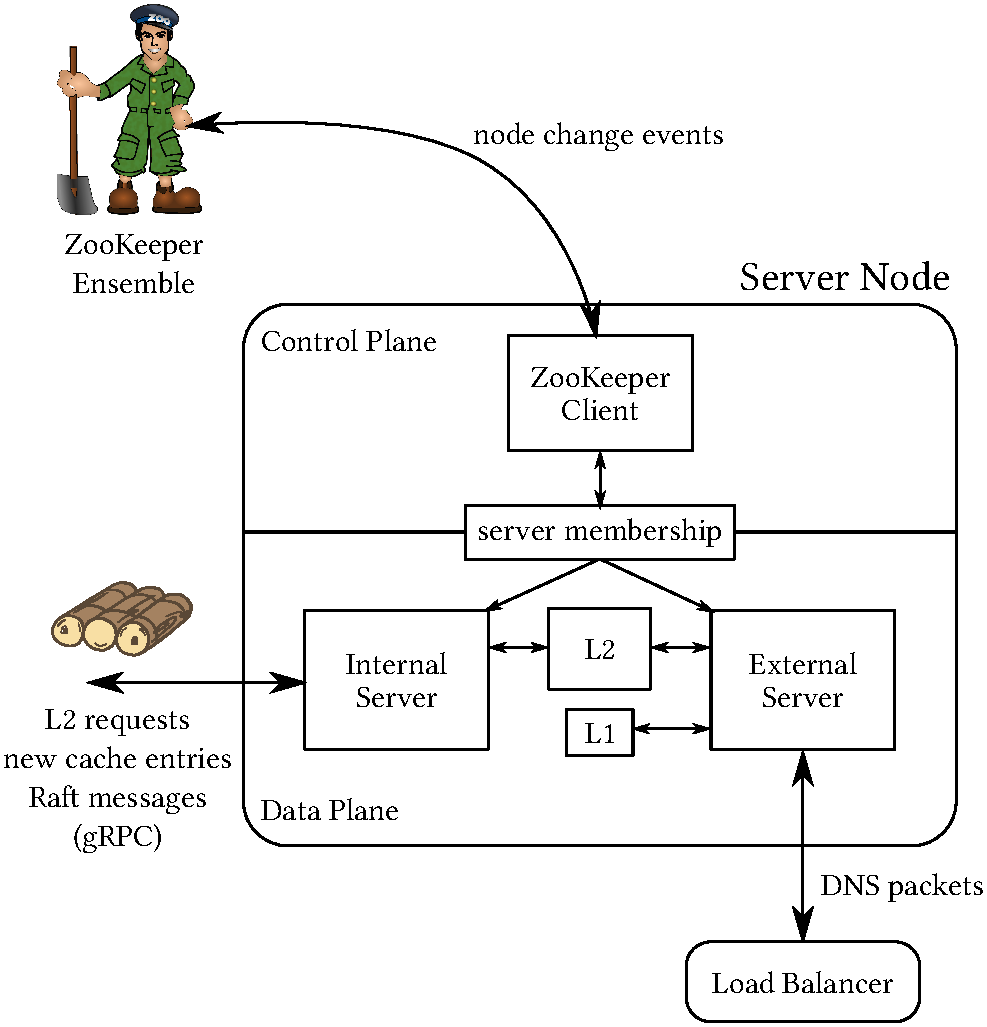
\includegraphics[width=0.35\textwidth]{internal.pdf}}
    \caption{Design of \dnszoo{}}
\vspace*{-\baselineskip}
\end{figure*}

\subsection{Overall Architecture}

The overall architecture of \dnszoo{} is depicted in \autoref{fig:overall}. It consists of three layers: the load balancer layer, the level 1 (L1) cache layer and the level 2 (L2) cache layer. The load balancer evenly distributes client requests to a group of servers that run our DNS service. The L1 layer is a small LFU cache local to each node that ideally contains popular DNS requests from all hash ranges. The L2 layer is a much larger cache partitioned by the request's hash value.

In case of a L1 cache miss, we partition the queries using its hash value and send it off to a designated L2 node. \dnszooch{} uses Consistent Hashing to divide up requests into buckets of server nodes, while \dnszoor{} uses a fixed set of Raft clusters as buckets. Membership in Consistent Hashing and Raft clusters is stored in ZooKeeper. The L2 cache is a replicated LRU cache in \dnszooch{} and a Raft-based key--value store in \dnszoor{}.

Now, we will walk through how a DNS request is served, which is shown in \autoref{fig:overall}. First, the client will send a request $r$ to the load balancer (step~1) which will distribute the request to one of the healthy servers (step~2). Assuming node $n$ received $r$, it will then check if $r$ hash exists in the L1 cache. If cache hit, $n$ will immediately return the result of $r$; otherwise it will check the node(s) responsible for $r$ and forwards $r$ to node $m$ that covers the hash range $r$ (step 3).\footnote{If $n$ happens to cover the hash range of $r$, then we set $m = n$.} Node $m$ will check its L2 cache and return the result immediately to node $n$ when there is a cache hit; otherwise, it will query an external DNS service, such as Cloudflare, to get and store the result (step 4) and then gossip it to a few other nodes in the same hash range (step 5). The result will then go from node $m$ to $n$ (step 6), the load balancer (step 7) and finally the client (step 8).

\subsection{Intra-node Organization}

We divide the tasks within a single server node into two logical \emph{planes,} as shown in \autoref{fig:internal}.

The \emph{Control Plane} is responsible for keeping the server membership up to date. Upon node startup, it communicates with the ZooKeeper ensemble to create ephemeral znodes that notify other nodes of its existence. It then reads the content of the directory containing \\
the ephemeral znodes to learn about other nodes in the system and to set up the bucketing strategy. In particular, it calls the \texttt{getChildren()} ZooKeeper API with the ``watch'' flag set to true, so that we receive future updates of the server membership.

The Control Plane exposes server membership information to the Data Plane, so that the lookup servers can accurately identify the L2 nodes to send a query to in case of a L1 cache miss.

The \emph{Data Plane} handles the actual DNS queries itself. It includes two servers, an Internal Server that exposes a gRPC service for inter-node communication, as well as an External Server that handles external DNS queries from the load balancer. Examples of inter-node communication include L2 queries, gossiped new cache entries (in \dnszooch{} only), and Raft proposals and heartbeats (in \dnszoor{} only). The Data Plane also includes the L1 and L2 caches. The External Server makes use of and updates both L1 and L2 caches, while the Internal Server only accesses the L2 cache.

In our implementation, each plane runs within its own goroutine (a lightweight threading construct in the Go programming language \cite{go}). However, the Control Plane goroutine is only actively running code at node startup, during server reconfigurations, and very occasionally through heartbeat messages. So the majority of CPU time is spent in the Data Plane applications as desired.

The separation of two planes has served us well. The well-defined and rigid interface between the two planes was beneficial for parallelizing our development process. It also effectively encapsulates the recovery mechanism, so that we may easily swap out ZooKeeper for another synchronization system as need be.

\subsection{Distributing Queries to Nodes} \label{sec:distribute-queries}
In both variants of \dnszoo{}, we rely on hashing to distribute DNS queries roughly uniformly among a set of buckets. However, the number of such buckets as well as the assignment of server nodes to each bucket constitute the most significant difference between \dnszooch{} and \dnszoor{}.

\paragraph{\textbf{Hashing the query}}
We have three requirements in determining an appropriate hash function for DNS queries:
\begin{enumerate}
    \item \emph{Speed.} Since \dnszoo{} is designed to have low latency and high throughput, the time it takes to hash a DNS query must be very short compared to completing a DNS request.
    \item \emph{Quality.} We rely on the hash function to distribute DNS queries evenly between buckets to reduce tail latency.
    \item \emph{Hash-flooding attack resistance.} It must be difficult to discover DNS queries that hash to the same bucket with high probability. If not, an adversary could flood \dnszoo{} with such queries, potentially overwhelming the nodes dedicated to that bucket \cite{2011hashdos}.
\end{enumerate}
On the other hand, we do \emph{not} need certain cryptographic properties like one-wayness.

We chose SipHash \cite{2012siphash} as it satisfies all our requirements. Our implementation currently hardcodes the hash key, but a future version of \dnszoo{} will store the hash key on ZooKeeper and rotate it periodically to better resist hash-flooding attacks.

We currently hash both the query type and query domain name together as it gives a better distribution for different queries. However, it is possible that storing different records for the same domain on the same node may improve locality. More work is needed to ascertain the tradeoffs of this alternative approach.

\paragraph{\textbf{Bucketing in \dnszooch{}}}
In \dnszooch{}, we use Consistent Hashing to map nodes to buckets, where each bucket is a hash range. Each node is assigned a fixed number of hash ranges, so the number of unique buckets increases along with the number of nodes. Conversely, each hash range is the responsibility of the top $Q$ nodes in the Consistent Hashing ring rather than just the top node. When one node updates its L2 cache in response to an incoming query, it gossips the new cache content to other nodes for the same hash range. Since the server membership set is stored in ZooKeeper and watched by all nodes, every update to the membership set is quickly known to every other node in the same order, so all nodes should have the same idea what the Consistent Hashing ring looks like at almost all times.

\paragraph{\textbf{Bucketing in \dnszoor{}}}
In \dnszoor{}, we use the most significant $n$ bits of the SipHash to map nodes to buckets where $n$ is a configurable number. More buckets should correspond to better load distribution on a large number of nodes. In this design, we implement a bucket management service, \textit{Hash Cluster Manager}, based on ZooKeeper for routing, load balancing and fault tolerance. The Hash Cluster Manager (HCM) will use ZooKeeper to elect a leader that assigns available hash buckets to available nodes. When a server dies, ZooKeeper will notify the leader about its death, who will in turn run the rebalancing algorithm to assign the new unassigned buckets to other servers. Each server monitors a pre-configured path on ZooKeeper and watches for potential assignments. All assignments are watched by all nodes so each server knows which node(s) to talk to when receiving an out-of-range DNS request that results in an L1 cache miss.

Each bucket corresponds to a multi-node Raft key--value store cluster that ensures fault tolerance and eventual consistency. Intra-server communication, including joining/exiting clusters and looking up cache values, is taken care of by gRPC.

\section{Implementation}
Both variants of \dnszoo{} are written exclusively in Go. Our entire service has over 5000 lines of Go code\footnote{Link to the repo: \url{https://github.com/TimothyGu/stanford-cs244B-project}}. The load balancing layer utilizes the AWS application load balancer, and the L1 layer is a simple LFU cache with a configurable size. Both layers are shared among the two difference approaches, so we will only discuss the L2 layer of \dnszooch{} and \dnszoor{}.

\subsection{\dnszooch{}}

For \dnszooch{}, we have two key components -- Consistent Hashing Membership Manager and the cache service.

\paragraph{\textbf{Consistent Hashing Membership Manager}} The consistent hashing membership manager shares a pre-configured ZooKeeper path \texttt{/chmembership} for membership management. Each node creates an ephemeral node with its node ID as the name and the gRPC service address as the value. All nodes monitor this path and adjust their hash ring accordingly. We do not need a leader in this case, and all functioning nodes operate independently and identically for membership changes.

\paragraph{\textbf{Cache Service}} The cache service is our L2 layer and consists of several small components -- the LRU cache and the Consistent Hashing ring. The LRU cache has a configurable size and serves as our implementation for the L2 cache. For the Consistent Hashing ring, we initialize the ring on all nodes with the same configurable partition counts, replication factor, and load factor, the last of which is a feature from the consistent hashing library we use that can distribute a node's hash range to other nodes to alleviate hot spot and load pressure.
% As we discussed in \autoref{sec:distribute-queries}, we utilize the membership information obtained from ZooKeeper to arrange the hash ring and get the next $Q$ candidate nodes on the ring. We also have the current server gossip DNS information via gRPC to some of its peers down the hash ring.


\subsection{\dnszoor{}} 

For \dnszoor{}, we also have two key components -- Hash Cluster Manager (HCM) and Raft Key--Value Store. 

\paragraph{\textbf{Hash Cluster Manager (HCM)}} The HCM leader has two main features:
\begin{enumerate}
    \item \emph{Leader election.} The HCM monitor group membership changes using ZooKeeper watches. When a node joins, it will create an ephemeral znode with the sequential flag on with the format $\mathit{node\-id}\_\allowbreak\mathit{seq\-num}$, and the content of which is that node's gRPC address. The leader will be the one with the smallest sequence number. Each node will watch the node with the largest sequence number $j$ smaller than its own $i$: $\max_{j < i} n_j$ where $n$ is the name of a node. When node $n$ has the smallest sequence number $i$, it becomes the leader.
    \item \emph{Hash bucket management.} The leader assigns available buckets to nodes that are below the designated load factor (number of Raft clusters it belongs to) and write the assignment to a persistent node-to-cluster znode in ZooKeeper.\footnote{We encountered a deadlock issue from the go-zookeeper library when adding multiple watches as sometimes it does not send events through the watch channels and resulting in the leader not getting notifications of children changes from the watch. This is not present in the \dnszooch{} implementation as we only have one watch for the entire service.}
    
    Each node (including the leader) monitors its own node-to-cluster znode. When it sees changes, it will exit or join the Raft clusters corresponding to removed or added buckets. It will acknowledge an assignment by creating an ephemeral znode with its own node ID under \texttt{/dns\-server/\allowbreak{}cluster2\-node/\allowbreak{}<cluster\-id>}.
    All nodes will monitor all cluster-to-node mappings to find out which node(s) to send to. We choose a random node from a Raft cluster to distribute loads within a fixed hash range in this case.
\end{enumerate}

\paragraph{\textbf{Raft Key--Value Store (Raft KVStore)}} The Raft KVStore is a distributed key--value store with eventual consistency guarantees. All nodes can respond to read and write requests, and only write requests require consensus. Therefore, you may get staled data when you query the wrong nodes, but it is very fast as all read requests are local, which satisfies our requirements for a highly available DNS service. The Raft protocol will commit a write or a delete request after reaching consensus, and individual KVStore will be able to read from Raft's committed log entries and apply them to the local map.

The Raft KVStore provides two gRPC APIs:
\begin{enumerate}
    \item $\mathtt{Cache} : (\mathtt{CacheRequest})\to\mathtt{CacheReply}$\\
    This API provides a way to specify whether it is a lookup, store or delete request and return results as soon as results are read from the local cache or update requests have been appended to the Raft log entries.
    \item $\mathtt{ConfChange} : (\mathtt{raftpb.ConfChange}) \to \mathtt{Empty}$\\
    This API allows individual nodes to join or exit a Raft cluster.
\end{enumerate}

\subsection{Key Libraries Used}
For Consistent Hashing, we utilize buraksezer's consistent library.\footnote{\url{https://github.com/buraksezer/consistent}} For Raft, we use etcd.io's implementation and base our key--value store heavily on their Raft kvstore example.\footnote{\url{https://github.com/etcd-io/etcd/tree/main/contrib/raftexample}} For ZooKeeper, we choose go-zookeeper's library.\footnote{\url{https://github.com/go-zookeeper/zk}} For DNS queries, we use miekg's DNS library.\footnote{\url{https://github.com/miekg/dns}}

\section{Evaluation}
We deployed \dnszooch{} on five \textsf{t2.micro} instances on Amazon EC2. Each instance has 1~CPU core and 1~GiB of RAM. Our ZooKeeper ensemble consists of a single \textsf{t3a.medium} EC2 instance with 1~CPU core and 4~GiB of RAM. We did not use multiple instances for ZooKeeper because our service uses ZooKeeper as an existing solution (black box) and we can easily deploy and configure multiple instances when needed. All EC2 instances reside in the same Availability Zone.

The testing setup is as following: we curate a list of active servers on ZooKeeper, start an EC2 instance as the client, and randomly choose a server from the list to send test requests to. In the future, we can use AWS application load balancer to distribute traffic across the available servers.

\subsection{Latency}
To measure the latency performance of the system, we generate random DNS queries using the top-100000-domains\footnote{\url{https://github.com/zer0h/top-1000000-domains}} database. We randomly select 2k unique domain names from the database. We set a popular domain ratio parameter $p\%$ to generate 10k requests with $1-p\%$ of the domain names making up $p\%$ of the requests and the rest $1-p\%$, to test if our system can demonstrate better performance when handling popular domain name requests. We define the latency as the interval between the time when the client sends the request and the time when it receives the response. We compare the performance with public DNS service providers such as Google (8.8.8.8) and Cloudflare (1.1.1.1). 

We also measure the node-to-node (intra EC2) and node-to-external (EC2 to the internet) latencies using ping 1000 on an EC2 instance (Table \ref{tab:latency1}), which should be the best-case scenario for latencies.
\begin{table}[ht] \centering \small
\vspace*{-0.2\baselineskip}
\begin{tabular}{@{}lrr@{}} \toprule
 & Avg Latency & 99.9\textsuperscript{th} Percentile \\ \midrule
Node-to-node & 0.5ms & 3.2ms \\
Node-to-external & 1.6ms & 20.4ms \\
\bottomrule
\end{tabular}
\caption{Latency Summary}
\label{tab:latency1}
\vspace*{-\baselineskip}
\end{table}

From \autoref{fig:alllatency}, we can see that by increasing the percentage of popular domains in our testing queries, the latencies comes down. This is expected because a higher ratio of popular domains better utilize our hierarchical caching structure. The average latencies are higher because of the 99th percentile latencies are higher, which is observed in public DNS services as well. This indicates that public offerings also cache popular domains. We can also see that in terms of the average latency, \dnszooch{} performs quite a bit better than Google's public DNS service, especially when queries do not contain a lot of popular domains. While Cloudflare is consistently quick, it is no match for \dnszooch{}. In terms of the 99th percentile latency, we can see that \dnszooch{} still leads, especially when the popular domain ratio is low. This indicates that our caching service is highly available, performing what we want it to do.
\begin{figure*}[ht]
\vspace*{-\baselineskip} 
\centering
\subcaptionbox{DNS Providers Latency Performance, 90th and 99th Percentile \label{fig:alllatency}}{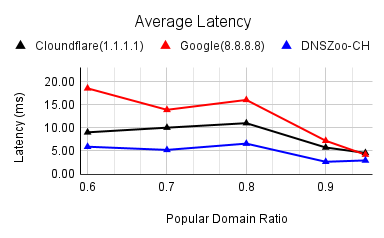
\includegraphics[width=0.3\textwidth]{avglatency.png}
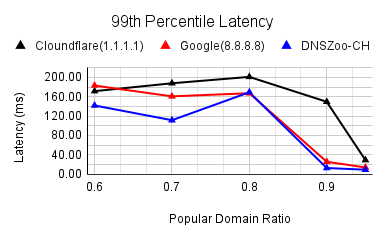
\includegraphics[width=0.3\textwidth]{all99pct.png}}

\subcaptionbox{\dnszooch{} Throughput and Scalability\label{fig:zoosc}}{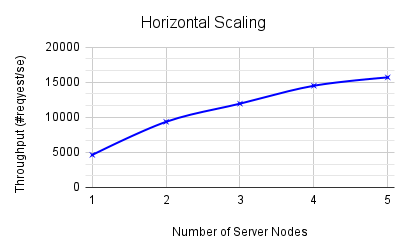
\includegraphics[width=0.3\textwidth]{scaling.png}}
\subcaptionbox{\dnszooch{} Fault Tolerance\label{fig:zooft}}{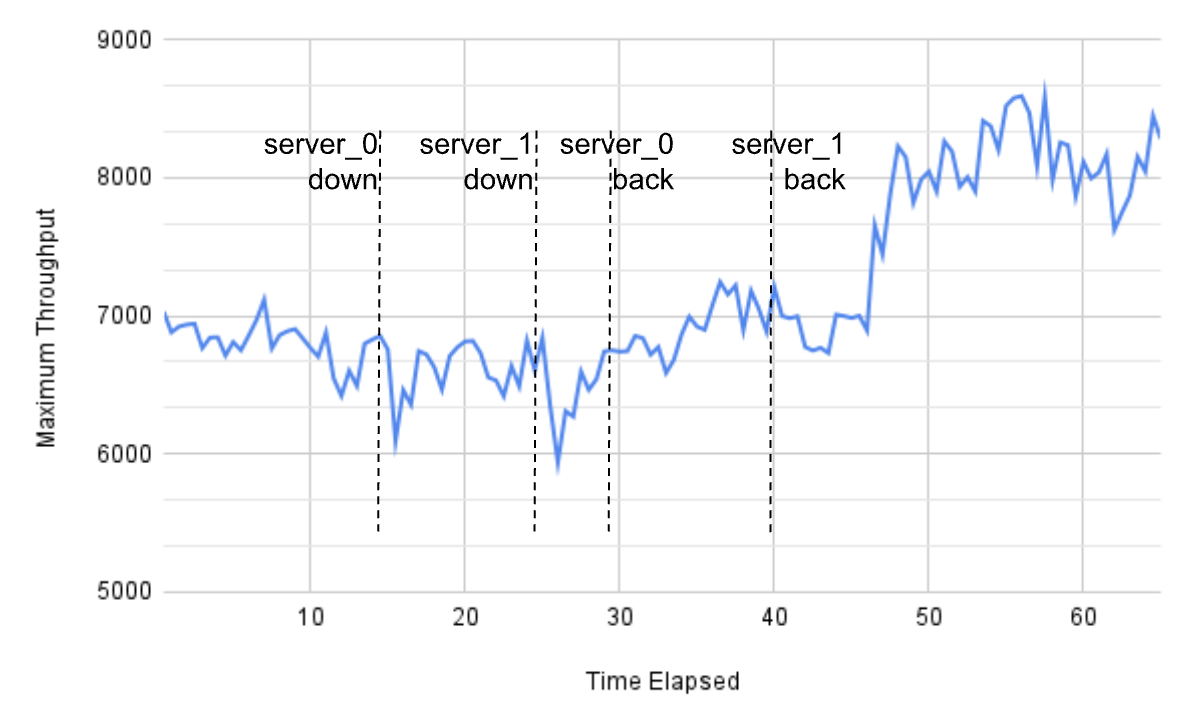
\includegraphics[width=0.3\textwidth]{fault.png}}

\caption{Various evaluation figures}
\vspace*{-\baselineskip}
\end{figure*}

\subsection{Throughput and Scalability}
We measure the throughput performance by sending a large number of requests to our system until the number of requests it can answer to in ten seconds reach a plateau. We then record the plateau number as its throughput. To issue a large number of queries, we start hundreds of go routines on the testing server, each of which sends requests sequentially using domain names from the top-100000-domains database. 

To measure the scalability of our system, we obtain its throughput with varying numbers of server nodes registered in ZooKeeper.

The result in \autoref{fig:zoosc} validates our design assumption and an almost-linear horizontal scalability of our system. 

\subsection{Fault Tolerance}
To measure the system's ability to tolerate server failures, we set up a test server that continuously sends requests of the number of the maximum throughput. Our system initially has four nodes. After the throughput number stabilizes, we shutdown two server nodes sequentially with an interval of about 10 seconds. We then bring back the two nodes in the same order. We monitor the system's throughput during the entire time frame and the result is recorded in \autoref{fig:zooft}.\\
The result proves that our system can withstand server failures. When the failure happens, our system will undergo a temporary drop of the throughput, but it can quickly recover to its maximum throughput prior to the failures. The reason why the throughput increases after the second server may be due to a consolidation of hash ranges on the surviving two nodes, which increases cache rate.

\section{Future Work}
We propose two different DNS server architecture designs, \dnszooch{} and \dnszoor{} in this paper and deploy \dnszooch{} on AWS EC2 and measure its performance. However, due to a deadlock issue from the go-zookeeper library, our \dnszoor{} design cannot fully function and thus cannot be tested, even though we expect it to perform better than \dnszooch{}. We would like to try to fix the deadlock issue from the ZK library, completing the implementation and compare its performance with \dnszooch{}.

In our current setup, users needs to obtain a list of available servers and manually round robin requests to those servers to mimick the behavior of a load balancer. We can easily use an AWS Load Balancer\footnote{\url{https://docs.aws.amazon.com/elasticloadbalancing/} and \url{https://aws.amazon.com/blogs/aws/new-application-load-balancing-via-ip-address-to-aws-on-premises-resources/}} to take care of this issue. We also need to integrate health monitoring of nodes into the load balancer to promptly remove slow, unresponsive or dead nodes from the AWS LB.

We introduce various parameters we can tune to further optimize the system performance:
\begin{itemize}
  \item L1 and L2 in-memory cache size: Increasing the size of L1 cache will benefit read requests for popular domains but also increase the overhead of managing expired records in L1 cache. 
  \item Partition count, replication factor and bounded load multiplier in the Consistent Hashing configuration.
\end{itemize}

We have validated the system performance on AWS EC2 to simulate a local area network. We are also interested in testing our system in a broader environment where server nodes are  geographically dispersed and compare their performances.

\section{Conclusion}
We manage to create a DNS caching service, \dnszoo{}, that consistently beats public offerings both in throughput and latency. \dnszoo{} also demonstrates almost-linear horizontal scalability and fault tolerance. We manage to design two completely different design approaches and succeed in completing one while the other one is blocked by a bug in the library we use. \dnszoo{} not only provides better throughput and latency than public DNS offerings, but also addresses the threat of getting throttled or banned by a public DNS service. Therefore, we believe \dnszoo{} will provide significant value frequent DNS querying is needed in a data center, for example, by web crawlers, and the design ideas of both \dnszooch{} and \dnszoor{} can be used in other applications. For example, consistent hashing can be used to distribute a search engine's indexing workload, and the Hash Cluster Manager can be tweaked to manage Kafka partitions in a distributed service.

% We design and implement a distributed DNS cache service with replicated cache in a hierarchical structure. Our system demonstrates high availability, horizontal scalability, and robustness to withstand server node failures. It supports instant server membership management to add and remove nodes dynamically. We propose a tailored design of load balancing strategy and consensus protocol in our system that relaxes the consistency requirement to achieve high availability and partition tolerance. The system is deployed and fully tested on Amazon EC2. We measure its latency, throughput and ability to tolerate node failures and validate it outperforms Google DNS service (8.8.8.8) on the latency metric in a local area network environment.

\bibliographystyle{ACM-Reference-Format}
\bibliography{main}


\end{document}
